
\section{Vectores}

\subsection{vectores}

 un vector es un ente matemático, es decir, es una figura creada para dar
    forma a la realidad como lo son la recta o el plano. Fue creada para
    representar fenómenos que no pueden ser descritos solamente con números, por
    ejemplo, la velocidad y las fuerzas. Son, por tanto, una construcción
    mas compleja que  la de los números y representan \textbf{una magnitud con
    dirección y sentido}. Gráficamente son representados como una recta con
    cierto ángulo de inclinación y un sentido marcado por una flecha, la
    dirección a la que apuntan.  Para poder representar un vector se necesitan
    al menos 2 puntos, el inicio del vector y el final (gráficamente, si unes 2
    puntos obtienes una recta, algebraicamente se restan $punto_{final}-
    punto_{inicial}=magnitud_{vector}$ )

    Existen muchos vectores,y estos son utilizados para dar representación a
    fenómenos físicos. En general un vector de dimensión $n$ es una tupla (un
    conjunto ordenado invariable de la forma $(x_1,x_2,\cdots,x_n)$ de números
    reales.

    Un vector posee 2 características:

    \begin{itemize} \item Modulo, es su valor, la longitud del segmento o la
                cantidad de espacios que se mueve en un determinado eje (o
                ejes).

        \item Dirección, En algunos textos se descompone como dirección y
            sentido.  Es el ángulo del segmento con respecto a un eje
            (normalmente x) y su sentido con respecto al origen (va o no hacia
            ese punto). Ejemplo: $29^o$ noreste sentido hacia arriba.
    \end{itemize}

    Gráficamente un vector de 2 dimensiones en el origen se ve de la forma:

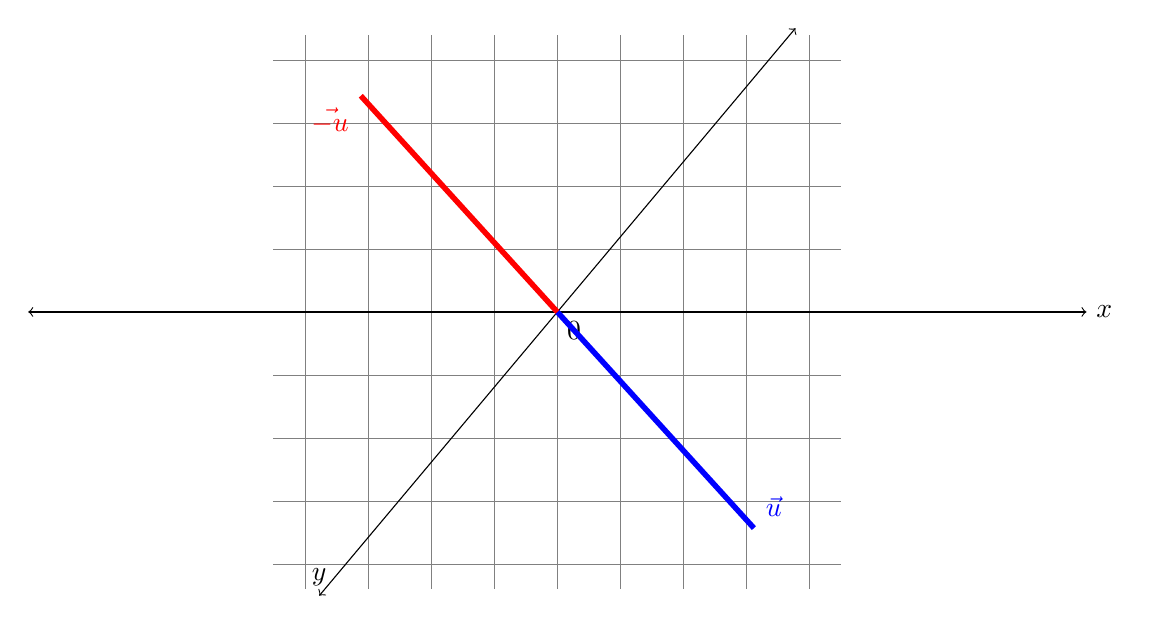
\begin{tikzpicture}[scale=1.6]

    \draw[style=help lines,step=0.5cm] (-4.1,-4.1)grid(4.1,4.1);

    \draw[<->] (-4.2,0)--(4.2,0) node[right]{$x$};
    \draw[<->] (0,-4.2)--(0,4.2) node[above]{$y$};
    \draw (0,0) node[anchor=north west ]{0};

    \draw[line width=2pt,blue](0,0)--(3,3.2) node[anchor=south west]{$\boldsymbol{\vec{u}}$};
    \draw[line width=2pt,red](0,0)--(-3,-3.2) node[anchor=north east]{$\boldsymbol{\vec{-u}}$};
\end{tikzpicture}

y de 3 dimensiones, en el origen se ve de la forma:


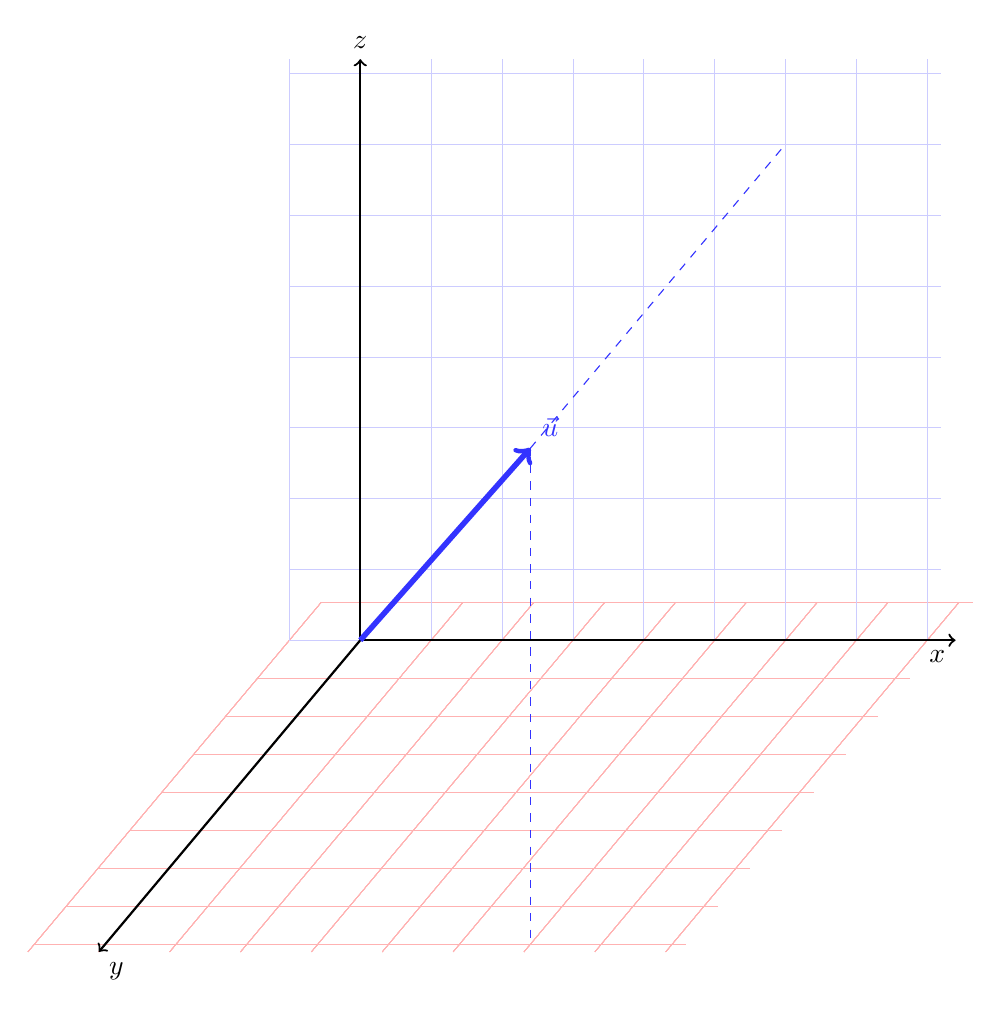
\begin{tikzpicture}[scale=1.8]
%standard tikz coordinate definition using x, y, z coords
    \coordinate (O) at (0,0,0);

\tikzset{
    x={(0:1cm)},y={(230:0.7cm)},z={(90:1cm)}
  }
 %draw a grid in the x-y plane
    \foreach \x in {-0.5,0,...,4}
        \foreach \y in {-0.5,0,...,4}
        {
            %eje xy
            \draw[very thin,red!30] (\x,-0.5) -- (\x,4.1);
            \draw[very thin,red!30] (-0.5,\y) -- (4.1,\y);
        }
%tikz-3dp %draw a grid in the x-z plane
    \foreach \x in {-0.5,0,...,4}
        \foreach \y in {0,0.5,...,4}
        {
            %eje xz
            \draw[very thin,blue!20] (\x,0,0) -- (\x,0,4.1);
            \draw[very thin,blue!20] (-0.5,0,\y) -- (4.1,0,\y);
        }
%draw axes
    \draw[->,thick] (0,0,0) -- (4.2,0,0) node[anchor=north east]{$x$};
    \draw[->,thick] (0,0,0) -- (0,4.1,0) node[anchor=north west]{$y$};
    \draw[->,thick] (0,0,0) -- (0,0,4.1) node[anchor=south]{$z$};

%draw a vector from O to P
    \draw[line width=2pt,blue!80,->] (O) -- (3,4,3.5)node[anchor=south west]{$\boldsymbol{\vec{u}}$};
    \draw[blue!80,dashed] (3,4,3.5)--(3,0,3.5);
    \draw[blue!80,dashed] (3,4,3.5)--(3,4,0);
\end{tikzpicture}




    Adicionalmente, los vectores poseen una \textbf{dimensión}, esta representa
    la cantidad de coordenadas las cuales cubre. Los vectores mas usados son
    los bidimensionales, que poseen 2 coordenadas, $X,Y$ y representan el plano
    o espacio bidimensional, son duplas ordenadas y pertenecen al espacio
    $\mathbb{R}^2$ y los tridimensionales, que utilizan 3 coordenadas $X,Y,Z$ y
    representan el espacio tridimensional perteneciendo al espacio
    $\mathbb{R}^3$.

    De igual forma, pueden utilizarse tantas dimensiones como hagan falta y el
    vector pertenecerá al espacio $\mathbb{R}^n$ donde $n$ es la cantidad de
    coordenadas que posee y es un numero natural.

    Cabe destacar que estos vectores también son muy utilizados ya que permiten
    extrapolar fenómenos físicos de mas variables, como por ejemplo el
    comportamiento de una caldera, o en el caso de 4 dimensiones cubrir también
    el tiempo $(x,y,z,t)$ y describir una fuerza o suceso en un espacio y
    tiempo determinado.

    Los vectores normalmente se utilizan para representar fuerzas, movimientos,
    variaciones, es decir cualquier condición física que implica una potencia o
    cambio ejercido en una dirección particular.

    Por simplificación, se trabajara en su mayoría con vectores en
    $\mathbb{R}^2$ y en $\mathbb{R}^3$ mas todos los conceptos son
    Extrapolables.

    Las operaciones, básicas, que se realizan con vectores son la suma
    algebraica, multiplicación por un escalar. Adicionalmente esta definida la
    multiplicación entre vectores como \textbf{producto punto} y
    \textbf{producto cruz}.

    \textbf{la división vectorial no esta definida!}, sin embargo, para ciertos
    tipos de vectores como fasores o números complejos se define una
    multiplicación y una división especial.



    \subsubsection{Representación}

    Los vectores pueden ser representados de 2 formas, mediante la descripción
    individual de sus características o mediante una magnitud y uno ángulos de
    referencia. Ambas formas de representación son equivalentes y se pueden
    llevar de una forma a otra.

    La forma de magnitud y ángulo suele ser utilizada para vectores en
    $\mathbb{R}^2$ y mas específicamente en un conjunto de vectores con propiedades
    adicionales como lo son los números complejos, ya que es fácil la
    transformación, el producto y la división definido \textbf{únicamente para
    ellos} y para representarlos solamente se necesita un
    ángulo. Para vectores de mayor dimensión suele usarse la representación por
    coordenadas, esto es debido a que para representar una linea en 3
    direcciones hacen falta al menos 2 ángulos, uno de giro horizontal y otro
    vertical (a esto se le conoce como coordenadas esféricas).


    \subsubsection{Representación en coordenadas rectangulares}

    Esta forma de representación se basa en descomponer el vector en los
    valores asociados que poseen en cada eje. Por ejemplo, si el vector es de
    $\mathbb{R}^2$ tiene coordenadas $x$ e $y$, por lo tanto el vector puede
    ser representado como la unión del origen (o un punto de referencia
    cualquiera) y los desplazamientos correspondientes en los ejes X,Y , si el
    vector es de 3 coordenadas, entonces serian X,Y,Z y así sucesivamente. A
    este tipo de coordenadas se le conocen como \textbf{ coordenadas
    cartesianas o rectangulares}.

    De esta forma, un vector puede escribirse de 2 formas, como tupla ordenada
    o como suma de componentes, en donde cada componente va a estar indicada
    por un \textbf{vector unitario}, el cual no es mas que una letra la cual
    indica a que eje corresponde; $\hat{\imath}$ para x, $\hat{\jmath}$ para y,
    $\hat{k}$ para k.

    De esta forma, un vector puede ser escrito de la forma:

    $$\vec{v}=(v_1,v_2,v_3,\cdots,v_n),\ v_i \in \mathbb{R}$$


    o de la forma:

    $$\vec{v}=v_1\cdot\hat{\imath}+v_2\cdot\hat{\jmath}+v_3\cdot\hat{k}+\cdots$$

    Gráficamente, estas composiciones son:

    Para 2 dimensiones:


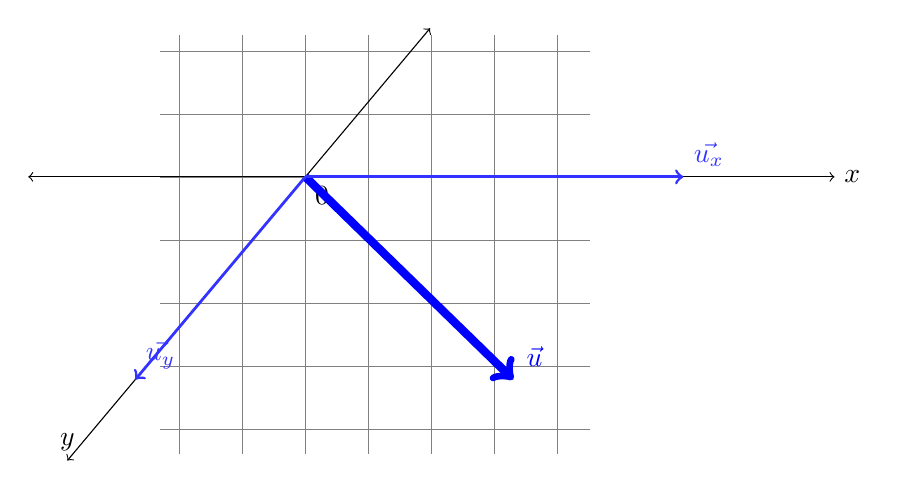
\begin{tikzpicture}[scale=1.6]
    \draw[style=help lines,step=0.5cm] (-2.1,-2.1)grid(4.1,4.1);
    \draw[<->] (-2.2,0)--(4.2,0) node[right]{$x$};
    \draw[<->] (0,-2.2)--(0,4.2) node[above]{$y$};
    \draw (0,0) node[anchor=north west ]{0};

    \draw[line width=3pt,blue,->](0,0)--(3,3) node[anchor=south west]{$\boldsymbol{\vec{u}}$};


    \draw[line width=1pt,blue!80,->](0,0)--(3,0) node[anchor=south west]{$\boldsymbol{\vec{u_x}}$};
    \draw[line width=1pt,blue!80,->](0,0)--(0,3) node[anchor=south west]{$\boldsymbol{\vec{u_y}}$};

\end{tikzpicture}

    Para 3 dimensiones:


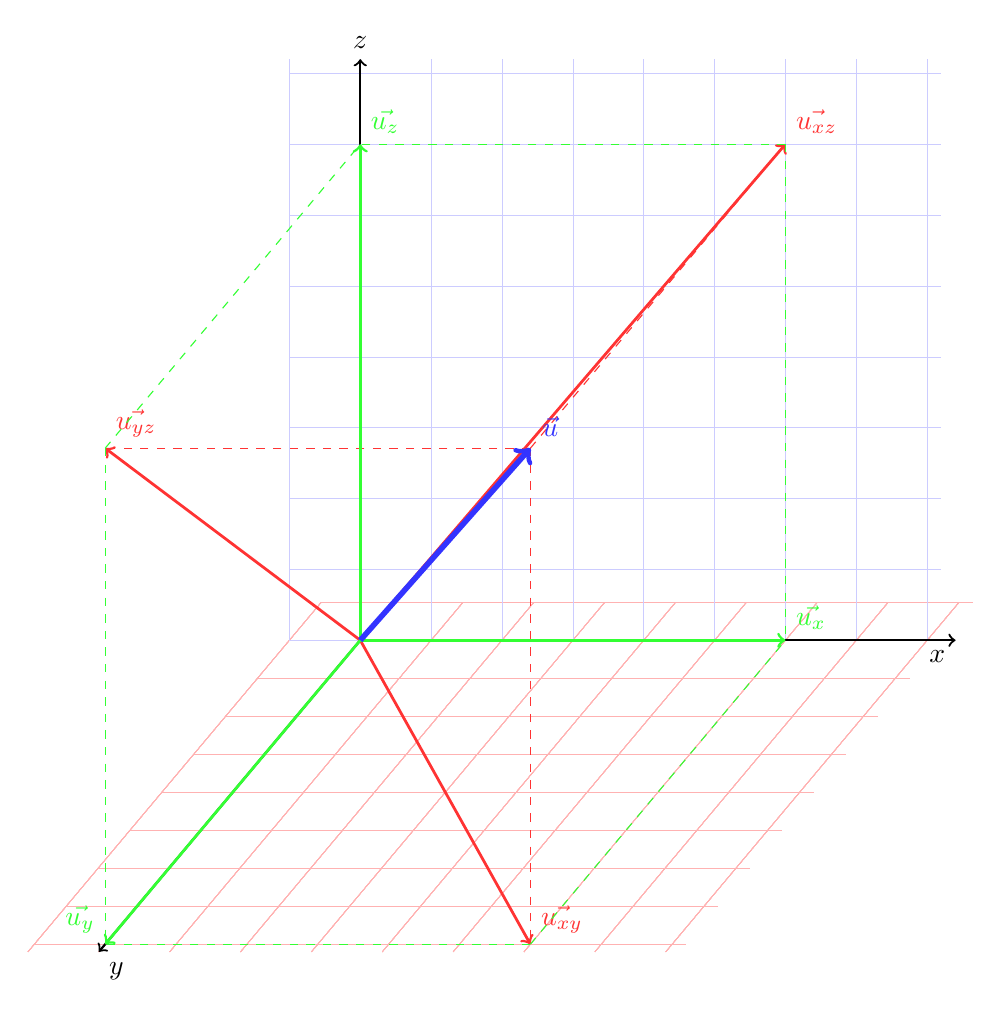
\begin{tikzpicture}[scale=1.8]
%standard tikz coordinate definition using x, y, z coords
    \coordinate (O) at (0,0,0);

\tikzset{
    x={(0:1cm)},y={(230:0.7cm)},z={(90:1cm)}
  }
 %draw a grid in the x-y plane
    \foreach \x in {-0.5,0,...,4}
        \foreach \y in {-0.5,0,...,4}
        {
            %eje xy
            \draw[very thin,red!30] (\x,-0.5) -- (\x,4.1);
            \draw[very thin,red!30] (-0.5,\y) -- (4.1,\y);
        }
%tikz-3dp %draw a grid in the x-z plane
    \foreach \x in {-0.5,0,...,4}
        \foreach \y in {0,0.5,...,4}
        {
            %eje xz
            \draw[very thin,blue!20] (\x,0,0) -- (\x,0,4.1);
            \draw[very thin,blue!20] (-0.5,0,\y) -- (4.1,0,\y);
        }
%draw axes
    \draw[->,thick] (0,0,0) -- (4.2,0,0) node[anchor=north east]{$x$};
    \draw[->,thick] (0,0,0) -- (0,4.1,0) node[anchor=north west]{$y$};
    \draw[->,thick] (0,0,0) -- (0,0,4.1) node[anchor=south]{$z$};

%draw a vector from O to P

    \draw[line width=1pt,red!80,->] (O) -- (0,4,3.5)node[anchor=south west]{$\boldsymbol{\vec{u_{yz}}}$} ;
    \draw[line width=1pt,red!80,->] (O) -- (3,0,3.5)node[anchor=south west]{$\boldsymbol{\vec{u_{xz}}}$} ;
    \draw[line width=1pt,red!80,->] (O) -- (3,4,0)node[anchor=south west]{$\boldsymbol{\vec{u_{xy}}}$} ;

    \draw[red!80,dashed] (3,4,3.5)--(3,0,3.5);
    \draw[red!80,dashed] (3,4,3.5)--(3,4,0);
    \draw[red!80,dashed] (3,4,3.5)--(0,4,3.5);

    \draw[line width=1pt,green!80,->] (O) -- (3,0,0)node[anchor=south west]{$\boldsymbol{\vec{u_{x}}}$} ;
    \draw[line width=1pt,green!80,->] (O) -- (0,4,0)node[anchor=south east]{$\boldsymbol{\vec{u_{y}}}$} ;
    \draw[line width=1pt,green!80,->] (O) -- (0,0,3.5)node[anchor=south west]{$\boldsymbol{\vec{u_{z}}}$} ;


    \draw[green!80,dashed] (3,0,3.5)--(0,0,3.5);
    \draw[green!80,dashed] (3,0,3.5)--(3,0,0);

    \draw[green!80,dashed] (0,4,3.5)--(0,4,0);
    \draw[green!80,dashed] (0,4,3.5)--(0,0,3.5);

    \draw[green!80,dashed] (3,4,0)--(3,0,0);
    \draw[green!80,dashed] (3,4,0)--(0,4,0);

    \draw[line width=2pt,blue!80,->] (O) -- (3,4,3.5)node[anchor=south west]{$\boldsymbol{\vec{u}}$} ;
\end{tikzpicture}




    Ejemplos:

    $$\vec{V}=(2,1)=2\hat{\imath}+1\hat{\jmath}$$
    $$\vec{V}=(-3,8)=-3\hat{\imath}+8\hat{\jmath}$$
    $$\vec{V}=(-21,-35)=-21\hat{\imath}-35\hat{\jmath}$$

    $$\vec{V}=(3,4,7)=3\hat{\imath}+4\hat{\jmath}+7\hat{k}$$
    $$\vec{V}=(-2,13,9)=-2\hat{\imath}+13\hat{\jmath}+9\hat{k}$$
    $$\vec{V}=(32,-4,-22)=32\hat{\imath}-4\hat{\jmath}-22\hat{k}$$


    \subsubsection{Representación en magnitud y ángulos}

    La otra forma de representar un vector es mediante una magnitud (que
    representa el tamaño del segmento-recta) y uno o mas ángulos, los cuales
    son tomados con respecto a un punto de referencia y permiten orientar el
    vector en el espacio. Este tipo de coordenadas es conocido como
    \textbf{coordenadas polares} para 2 variables-ejes y \textbf{coordenadas
    esféricas} para 3 variables-ejes. Se escribe de la forma:

    $$\vec{V}= magnitud \phase{\theta} $$
    $$\vec{V}= magnitud  \phase{\theta}\phase{\phi} $$

    Donde, $magnitud$ se suele representar con la letra $r$ y los ángulos
    suelen venir expresados en grados, además, $\theta$ mide el plano XY y
    $\phi$ el ángulo con el eje Z. Y están limitados por:


     \begin{align*}
         0\leq r&<\infty & 0\leq\theta&<2\pi & 0\leq\phi&\leq\pi \\
         0\leq r&<\infty & 0^\circ\leq\theta&<360^\circ & 0^\circ\leq\phi&\leq180^\circ
    \end{align*}

    Cabe resaltar que la nomenclatura puede variar y en algunos textos $\theta$
    se cambia por $\phi$, esto es debido a una falta de estandarización (como los
    cm y pulgadas, kg y libras, etc) en este texto se utilizara la convención
    antes descrita para evitar confusiones, ya que en polares se usa $\theta$ para
    el plano XY.

    Ejemplos:


    $$\vec{V}=12 \phase{38^\circ} $$
    $$\vec{V}=23,22 \phase{98^\circ} $$
    $$\vec{V}=87,9 \phase{128^\circ} $$

    $$\vec{V}=45 \phase{12^\circ}\phase{30^\circ} $$
    $$\vec{V}=5 \phase{342^\circ}\phase{120^\circ} $$
    $$\vec{V}=23 \phase{2^\circ}\phase{180^\circ} $$

    Ambas representaciones son equivalentes,y esta equivalencia se logra
    mediante la trigonometría, mas específicamente un triangulo rectángulo.



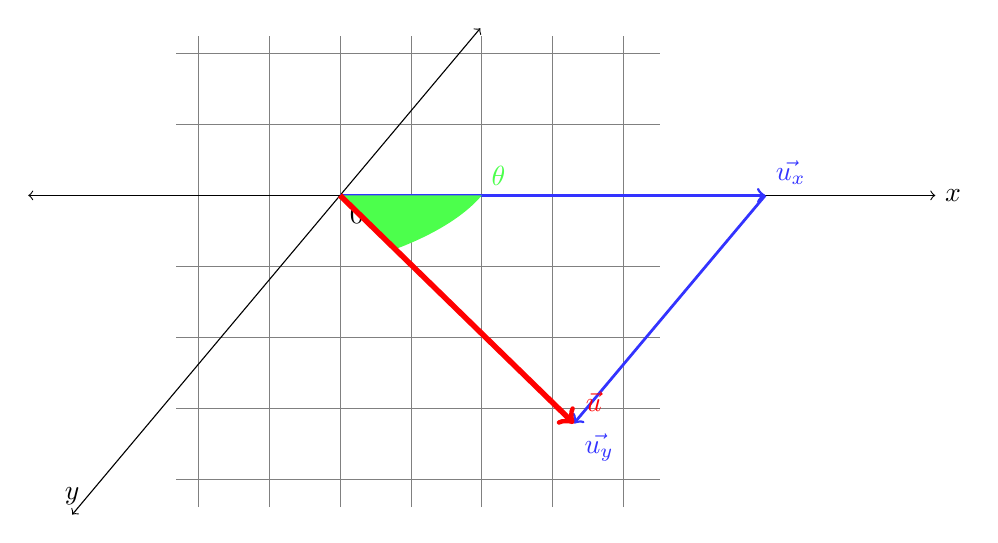
\begin{tikzpicture}[scale=1.8]
    \draw[style=help lines,step=0.5cm] (-2.1,-2.1)grid(4.1,4.1);
    \draw[<->] (-2.2,0)--(4.2,0) node[right]{$x$};
    \draw[<->] (0,-2.2)--(0,4.2) node[above]{$y$};
    \draw (0,0) node[anchor=north west ]{0};


    \draw[line width=1pt,blue!80,->](0,0)--(3,0) node[anchor= south west]{$\boldsymbol{\vec{u_x}}$};
    \draw[line width=1pt,blue!80,->](3,0)--(3,3) node[anchor=north  west]{$\boldsymbol{\vec{u_y}}$};
    \fill[green!70] (0,0)--(1,0) node[anchor=south west]{$\theta$} -- (1,0)  arc [start angle=0,end angle=45,x radius=1, y radius=1] ;

    \draw[line width=2pt,red,->](0,0)--(3,3) node[anchor=south west]{$\boldsymbol{\vec{u}}$};
\end{tikzpicture}


\tdplotsetmaincoords{60}{110}
\begin{tikzpicture}[scale=1.8,tdplot_main_coords]
%standard tikz coordinate definition using x, y, z coords
    \coordinate (O) at (0,0,0);

\tikzset{
    x={(0:1cm)},y={(230:0.7cm)},z={(90:1cm)}
  }
 %draw a grid in the x-y plane
    \foreach \x in {-0.5,0,...,4}
        \foreach \y in {-0.5,0,...,4}
        {
            %eje xy
            \draw[very thin,red!30] (\x,-0.5) -- (\x,4.1);
            \draw[very thin,red!30] (-0.5,\y) -- (4.1,\y);
        }
%tikz-3dp %draw a grid in the x-z plane
    \foreach \x in {-0.5,0,...,4}
        \foreach \y in {0,0.5,...,4}
        {
            %eje xz
            \draw[very thin,blue!20] (\x,0,0) -- (\x,0,4.1);
            \draw[very thin,blue!20] (-0.5,0,\y) -- (4.1,0,\y);
        }
%draw axes
    \draw[->,thick] (0,0,0) -- (4.2,0,0) node[anchor=north east]{$x$};
    \draw[->,thick] (0,0,0) -- (0,4.1,0) node[anchor=north west]{$y$};
    \draw[->,thick] (0,0,0) -- (0,0,4.1) node[anchor=south]{$z$};

%draw a vector from O to P

    \draw[red!80,dashed] (3,4,3.5)--(3,4,0);

    \begin{scope}[canvas is xy plane at z=0, thick]
        \draw (1,0) arc (0:53.13:1) ;
        \draw (1,0) node[anchor=north west ]{$\theta$};
    \end{scope}

    \tdplotsetthetaplanecoords{53.13}
    \tdplotdrawarc[tdplot_rotated_coords]{(0,0,0)}{1}{0}{40.5729}{anchor=south west}{$\phi$}

    \draw[line width=1pt,red!80,->] (O) -- (3,4,0)node[anchor=south west]{$\boldsymbol{\vec{u_{xy}}}$} ;
    \draw[line width=2pt,blue!80,->] (O) -- (3,4,3.5)node[anchor=south west]{$\boldsymbol{\vec{u}}$} ;
\end{tikzpicture}


    Como se observa en la imagen, y se sabe de la representación por
    coordenadas, un vector puede representarse como sus coordenadas en los
    ejes, estas representaciones forman los catetos del triangulo y la magnitud
    total representa la hipotenusa del mismo. De esta forma, se tiene que:

    Para 2 variables:

    polares a cartesianas
    $$\vec{V_x}= r\cdot cos(\theta)$$
    $$\vec{V_y} =  r\cdot sen(\theta)$$

    cartesianas a polares
    $$ r = \sqrt{V_x ^2+v_y^2}$$
    $$\theta= arctan\left(\frac{V_y}{V_x}\right)$$



    para3 variables:

    esféricas a cartesianas
    $$\vec{V_x}= r\cdot cos(\theta) \cdot sin(\phi)$$
    $$\vec{V_y} = r\cdot sen(\theta)\cdot sin(\phi)$$
    $$\vec{V_z}=r\cdot cos(\phi)$$

    cartesianas a esféricas
    $$ r = \sqrt{V_x ^2+v_y^2+v_z^2}$$
    $$\theta= arctan\left(\frac{V_y}{V_x}\right)$$
    $$\phi = arcos\left(\frac{V_z}{r}\right)$$


    Ejemplos:


    Transformar a polares:

     \begin{align*}
         \vec{V}&=(2,1) \\
         r &= \sqrt{2^2+1^2}  \rightarrow r= \sqrt{5} \\
         \theta&= arctan\left(\frac{1}{2}\right)  \rightarrow \theta= 26,57 ^\circ \\
    \end{align*}

     \begin{align*}
         \vec{V}&=(-3,8) \\
         r &= \sqrt{(-3)^2+8^2} \rightarrow r= \sqrt{73} \\
         \theta&= arctan\left(\frac{8}{-3}\right)  \rightarrow \theta= -69,44^\circ =-69,44^\circ+360^\circ=290.56 \\
    \end{align*}

     \begin{align*}
         \vec{V}&=(-21,-35) \\
         r &= \sqrt{(-21)^2+(-35)^2}  \rightarrow r= 7\sqrt{34} \\
         \theta&= arctan\left(\frac{-35}{-21}\right)  \rightarrow \theta= 59,04^\circ\\
    \end{align*}

    Transformar a esféricas:

    \begin{align*}
        \vec{V}&=(3,4,7) \\
        r &= \sqrt{3^2+4^2+7^2} \rightarrow w =\sqrt{74}  \\
        \theta&= arctan\left(\frac{4}{3}\right)  \rightarrow \theta= 53,13^\circ \\
        \phi &=arcos\left(\frac{7}{\sqrt{74}}\right)  \rightarrow \phi= 35,54^\circ\\
    \end{align*}

    \begin{align*}
        \vec{V}&=(-2,13,9) \\
        r &= \sqrt{(-2)^2+13^2+9^2}  \rightarrow w =\sqrt{254}  \\
        \theta&= arctan\left(\frac{13}{-2}\right)  \rightarrow \theta= -81,25^\circ= 278.75^\circ\\
        \phi &= arcos\left(\frac{9}{\sqrt{254}}\right)  \rightarrow \phi=  55,62^\circ\\
    \end{align*}

    \begin{align*}
        \vec{V}&=(32,-4,-22) \\
        r &= \sqrt{32^2+(-4)^2+22^2}  \rightarrow w =2\sqrt{381}  \\
        \theta&= arctan\left(\frac{13}{-2}\right)  \rightarrow \theta= -7,13^\circ=352,87^\circ \\
        \phi &= arcos\left(\frac{-22}{2\sqrt{381}}\right)  \rightarrow \phi= 124,3^\circ\\
    \end{align*}

    Transformar a rectangulares
    \begin{align*}
        \vec{V}&=12\phase{38^\circ}  \\
        \vec{V_x}&= 12\cdot cos(38^\circ) \rightarrow \vec{V_x} = \sqrt{9,456} \\
        \vec{V_y}& =  12\cdot sen(38^\circ)  \rightarrow \vec{V_y}= \sqrt{7,388} \\
    \end{align*}

    \begin{align*}
        \vec{V}&=23,22 \phase{98^\circ}  \\
        \vec{V_x}&= 23,22\cdot cos(98^\circ)  \rightarrow \vec{V_x} = \sqrt{18,298} \\
        \vec{V_y}& =  23,22\cdot sen(98^\circ)  \rightarrow \vec{V_y}= \sqrt{14.296} \\
    \end{align*}

    \begin{align*}
        \vec{V}&=87,9 \phase{128^\circ}  \\
        \vec{V_x}&= 87,9\cdot cos(128^\circ) \rightarrow \vec{V_x} = \sqrt{-54,117} \\
        \vec{V_y}& =  87,9\cdot sen(128^\circ)  \rightarrow \vec{V_y}= \sqrt{69.266} \\
    \end{align*}


    \begin{align*}
        \vec{V}&=45 \phase{12^\circ}\phase{30^\circ} \\
        \vec{V_x}&= 45\cdot cos(12^\circ) \cdot sin(30^\circ)  \rightarrow \vec{V_x} = \sqrt{22,008} \\
        \vec{V_y} &= 45\cdot sen(12^\circ)\cdot sin(30^\circ) \rightarrow \vec{V_x} = \sqrt{4,678} \\
        \vec{V_z}&=45\cdot cos(30^\circ)  \rightarrow \vec{V_x}= \sqrt{38,971} \\
    \end{align*}

    \begin{align*}
        \vec{V}&=5 \phase{342^\circ}\phase{120^\circ}\\
        \vec{V_x}&= 5\cdot cos(342^\circ) \cdot sin(120^\circ)   \rightarrow \vec{V_x} = \sqrt{4,118} \\
        \vec{V_y} &=5r\cdot sen(342^\circ)\cdot sin(120^\circ)  \rightarrow \vec{V_x} = \sqrt{-1,338} \\
        \vec{V_z}&=5\cdot cos(120^\circ)  \rightarrow \vec{V_x} = \sqrt{-2,5} \\
    \end{align*}

    \begin{align*}
        \vec{V}&=23 \phase{0^\circ}\phase{180^\circ}\\
        \vec{V_x}&= 23\cdot cos(2^\circ) \cdot sin(180^\circ)   \rightarrow \vec{V_x} = \sqrt{0} \\
        \vec{V_y} &= 23\cdot sen(2^\circ)\cdot sin(180^\circ)  \rightarrow \vec{V_x} = \sqrt{0} \\
        \vec{V_z}&= 23\cdot cos(180^\circ)  \rightarrow \vec{V_x} = \sqrt{-23} \\
    \end{align*}


    \subsubsection{Suma}

    La suma de vectores se realiza con los vectores en su forma cartesiana, es
    decir,\textbf{ para poder sumar 2 vectores debemos llevarlo a su forma
    rectangular}, La forma en la que se hace la suma es simplemente sumar sus
    componentes internas, es decir su representación en $x$ con su respectivo
    par, la de $y$ con $y$ y así sucesivamente.

    Sean $\vec{v},\vec{u}$ dos vectores cualesquiera de $\mathbb{R}^n$ tal que:

    $$\vec{v}=(v_1,v_2,v_3,\cdots,v_n)\ ; \vec{u}=(u_1,u_2,u_3,\cdots,u_n)$$
    $$\vec{r}=\vec{v+u}=(v_1+u_1,v_2+u_2,v_3+u_3,\cdots,v_n+u_n)$$

    \textbf{Recuerde que,} una suma algebraica es la suma con signo de los
    elementos, esto quiere decir que incluye a la resta ya que si se suman
    números de signos opuestos es lo mismo a restarlos.

    Gráficamente, la forma mas sencilla es dibujar el primer vector en el
    origen y en su extremo dibujar el siguiente vector (el que se le sumara
    algebraicamente), luego se unen el origen del primer vector (corresponde
    con el origen del plano por como se definió) y el fin del segundo vector
    y este es el vector suma resultante.

    Gráficamente, para $\mathbb{R}^2$:


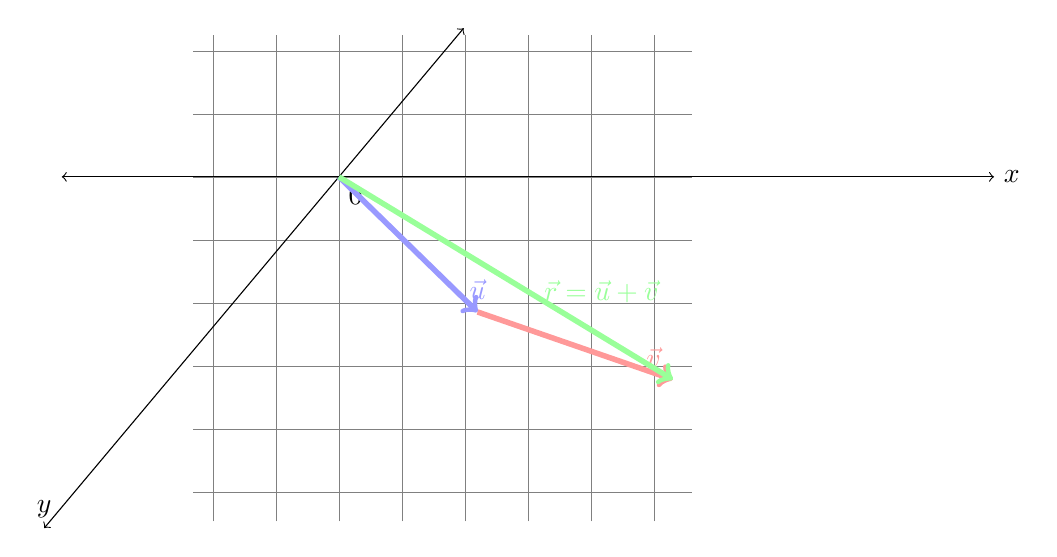
\begin{tikzpicture}[scale=1.6]
    \draw[style=help lines,step=0.5cm] (-2.1,-2.1)grid(5.1,5.1);
    \draw[<->] (-2.2,0)--(5.2,0) node[right]{$x$};
    \draw[<->] (0,-2.2)--(0,5.2) node[above]{$y$};
    \draw (0,0) node[anchor=north west ]{0};

    \draw[line width=2pt,blue!40,->](0,0)--(2,2) node[anchor=south]{$\boldsymbol{\vec{u}}$};

    \draw[line width=2pt,red!40,->](2,2)--(4,3) node[anchor=south east ]{$\boldsymbol{\vec{v}}$};

    \draw[line width=2pt,green!40,->](0,0)--(4,3) ;
    \draw[line width=2pt,green!40] (2.3,1.7) node[anchor=west ]{$\boldsymbol{\vec{r}=\vec{u}+\vec{v}}$};
\end{tikzpicture}

    Ejemplos: Sumar los siguientes vectores

    \begin{align*}
        \vec{V}& =(2,1) \ \ ;\ \ \ \vec{U} =(-3,8)		\\
        \vec{R}&= (2-3 ,1+8 )   \rightarrow \vec{R} = (-1 ,9  )
    \end{align*}

    \begin{align*}
        \vec{V}& =(-21,-35)  \ \ ;\ \ \  \vec{U} =(-3,8)		\\
        \vec{R}&= (-21-3 ,-35+8  )  \rightarrow \vec{R} = (-24 ,-27  )
    \end{align*}

    \begin{align*}
        \vec{V}& =(-21,-35)  \ \ ;\ \ \  \vec{U} =(2,1)		\\
        \vec{R}&= (-21+2 , -35+1 )   \rightarrow \vec{R} = (-19 ,-34  )
    \end{align*}




    \begin{align*}
        \vec{V}& =(3,4,7)  \ \ ;\ \ \   \vec{U} =(-2,13,9)		\\
        \vec{R}&= (3-2 ,4+13 ,7+9 )   \rightarrow \vec{R} = (4,17,16 )
    \end{align*}

    \begin{align*}
        \vec{V}& =(3,4,7)  \ \ ;\ \ \  \vec{U} =(32,-4,-22)		\\
        \vec{R}&= (3+32, 4-4,7-22 )  & \rightarrow \vec{R} &= ( 35,0 ,-15 )
    \end{align*}

    \begin{align*}
        \vec{V}& =(-2,13,9)  \ \ ;\ \ \   \vec{U} =(32,-4,-22)		\\
        \vec{R}&= (-2+32 ,13-4 ,9-22 )  \rightarrow \vec{R} = (30, 9,-13 )
    \end{align*}


    \subsubsection{Producto por escalar}

    El producto por escalar es una operación que toma un vector cualesquiera
    $\vec{v} \in \mathbb{R}^n$ y un escalar (numero) cualquiera $\alpha \in
    \mathbb{R}$. Consiste en multiplicar ese escalar por todos los elementos del
    vector modificando de esta forma su magnitud. Cuando el vector se encuentra
    en coordenadas polares o esféricas solamente se modifica la magnitud,
    multiplicándola por el escalar, el ángulo permanece igual.

    Sean $\vec{v}$ un  vector cualesquiera de $\mathbb{R}^n$  tal que:

    $$\vec{v}=(v_1,v_2,v_3,\cdots,v_n)\ ; \alpha \in \mathbb{R} $$
    $$\vec{r}=\alpha\cdot\vec{v}=(v_1\cdot\alpha,v_2\cdot\alpha,v_3\cdot\alpha,\cdots,v_n\cdot\alpha)$$

    Gráficamente:
    \begin{itemize}
        \item Aumenta su tamaño si $|\alpha| >1$.
        \item Reduce su tamaño si $|\alpha| <1$.

        \item Invierte su dirección y  sigue las reglas de la magnitud anteriores
            si $\alpha<0$.

        \item Permanece igual si $\alpha=1$.
        \item Se anula se $\alpha = 0$.
    \end{itemize}


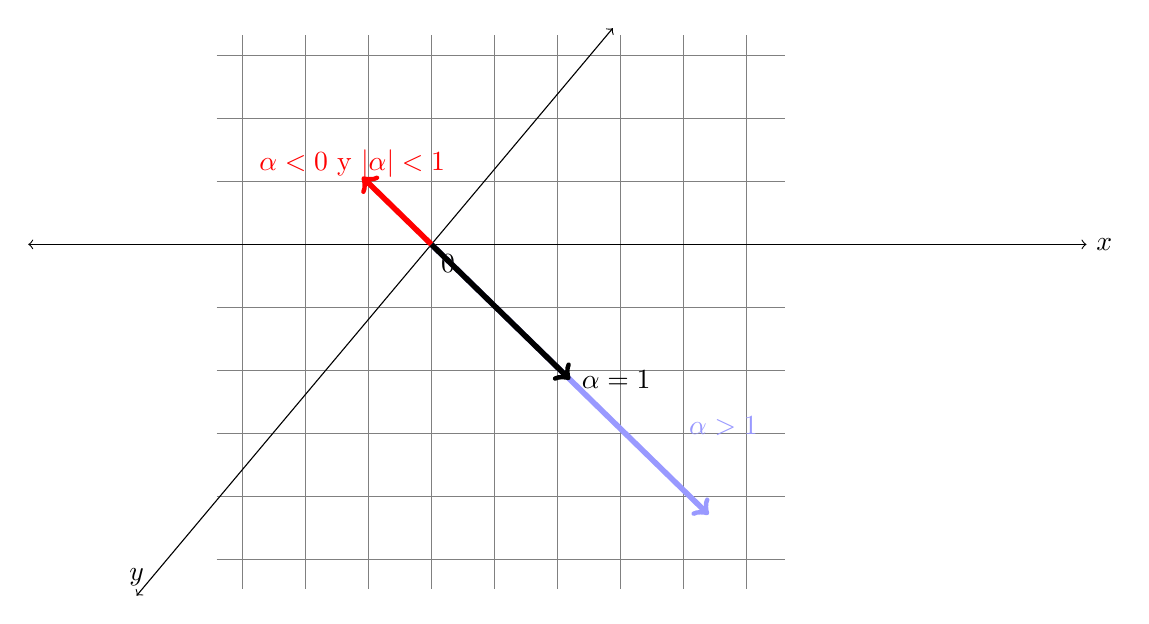
\begin{tikzpicture}[scale=1.6]
    \draw[style=help lines,step=0.5cm] (-3.1,-3.1)grid(5.1,5.1);
    \draw[<->] (-3.2,0)--(5.2,0) node[right]{$x$};
    \draw[<->] (0,-3.2)--(0,5.2) node[above]{$y$};
    \draw (0,0) node[anchor=north west ]{0};

    \draw[line width=2pt,blue!40,->](0,0)--(4,4) ;
    \draw[line width=2pt,blue!40] (3.3,3) node[anchor=south west]{$\alpha>1$};

    \draw[line width=2pt,red,->](0,0)--(-1,-1) ;
    \draw[line width=2pt,red] (-2,-1.2) node[anchor=west ]{$\alpha<0$ y $|\alpha|<1$};

    \draw[line width=2pt,->](0,0)--(2,2) node[anchor=west]{$\alpha=1$};
\end{tikzpicture}


    Ejemplos, multiplicar los siguientes vectores por los escalares:

    \begin{align*}
        \vec{V}& =(2,1)  \ \ ;\ \ \  \alpha =3 		\\
        \vec{R}&= (2\times3,1\times3 )   \rightarrow \vec{R}= (6,3 )
    \end{align*}

    \begin{align*}
        \vec{V}& =(-3,8)  \ \ ;\ \ \  \alpha = 8		\\
        \vec{R}&= (-3 \times8,8 \times8 )   \rightarrow \vec{R}= (-24,64 )
    \end{align*}

    \begin{align*}
        \vec{V}& =(-21,-35)  \ \ ;\ \ \ \alpha = -5		\\
        \vec{R}&= (-21 \times-5,-35 \times-5)  \rightarrow \vec{R} = (105,175 )
    \end{align*}





    \begin{align*}
        \vec{V}& =(3,4,7)  \ \ ;\ \ \  \alpha= -9	\\
        \vec{R}&= (3 \times-9,4 \times-9,7 \times-9  )  \rightarrow \vec{R}= (-27,-36,-63 )
    \end{align*}

    \begin{align*}
        \vec{V}& =(-2,13,9)  \ \ ;\ \ \  \alpha = 12 		\\
        \vec{R}&= (-2 \times12, 13 \times12, 9 \times12)  \rightarrow \vec{R}= (-24,156,108)
    \end{align*}

    \begin{align*}
        \vec{V}& =(32,-4,-22)  \ \ ;\ \ \  \alpha = -1		\\
        \vec{R}&= (32 \times-1, -4 \times-1, -22 \times-1 )  \rightarrow \vec{R}= (-32,4,22)
    \end{align*}




    \subsubsection{Multiplicación entre vectores}

    La multiplicación entre vectores es una propiedad definida de una forma
    muy distinta a la multiplicación numérica. Esto se debe a la complejidad de
    los vectores la cual permite definí varios tipos de multiplicaciones posibles
    las cuales tienen sentido. Las 2 Multiplicaciones mas conocidas son \textbf{
    el producto punto y el producto cruz}, además de esto existen otras formas
    de realizar multiplicaciones como la es la de los números complejos, siendo
    esta definida de tal forma que permite incluso crear una división.

    Los producto punto y producto cruz \textbf{No tienen operación inversa} y es
    por esto que \textbf{no existe la división vectorial}.

    \subsubsection{Producto punto}

    Este tipo de multiplicación es realizable par todos los vectores y da como
    resultado un escalar, es decir un numero.

    Se escribe de la forma: $\vec{r} = \vec{v}\cdot\vec{u}$, con
    $\vec{v},\vec{u}$ vectores cualesquiera.

    La forma de definir este producto varia, existen varios procedimientos
    equivalentes, las dos mas conocidas son con la norma de cada uno de los vectores
    y el ángulo entre vectores, y el que se trabajara acá que es una suma del
    producto entre los componentes del vector. Es decir:

    Sean $\vec{v},\vec{u}$ dos vectores cualesquiera de $\mathbb{R}^n$ tal que:

    \begin{align*}
        \vec{v}&=(v_1,v_2,v_3,\cdots,v_n) \ \ ;\ \ \ \vec{u}=(u_1,u_2,u_3,\cdots,u_n)\\
        \vec{r}&=\vec{v}\cdot\vec{u}= (v_1\cdot u_1,v_2 \cdot u_2,v_3 \cdot u_3,\cdots,v_n \cdot u_n)\rightarrow
        \vec{r}= \sum_{i=0}^{n} v_i\cdot u_i
    \end{align*}


    Ejemplos:

    \begin{align*}
        \vec{V}& =(2,1) \ \ ;\ \ \  \vec{U} =(-3,8)		\\
        \vec{R}&= 2\cdot-3 +1\dot8   \rightarrow \vec{R}= 2
    \end{align*}

    \begin{align*}
        \vec{V}& =(-21,-35)  \ \ ;\ \ \  \vec{U} &=(-3,8)		\\
        \vec{R}&= -21\cdot-3 +\ -35\cdot8    \rightarrow \vec{R}= -217
    \end{align*}

    \begin{align*}
        \vec{V}& =(-21,-35)  \ \ ;\ \ \ \vec{U} &=(2,1)		\\
        \vec{R}&= -21\cdot2 + -35\cdot1   \rightarrow \vec{R}= -77
    \end{align*}




    \begin{align*}
        \vec{V}& =(3,4,7)   \ \ ;\ \ \  \vec{U} =(-2,13,9)		\\
        \vec{R}&= 3\cdot-2 +4\cdot13 +7\cdot9   \rightarrow \vec{R} = 109
    \end{align*}

    \begin{align*}
        \vec{V}& =(3,4,7)  \ \ ;\ \ \  \vec{U} =(32,-4,-22)		\\
        \vec{R}&= 3\cdot32 + 4\cdot-4 +7\cdot22    \rightarrow \vec{R} = -74
    \end{align*}

    \begin{align*}
        \vec{V}& =(-2,13,9)  \ \ ;\ \ \   \vec{U} =(32,-4,-22)		\\
        \vec{R}&= -2\cdot32 + 13\cdot-4 +9\cdot-22 )  \rightarrow \vec{R} = -314
    \end{align*}

    \subsubsection{Producto cruz}

    Este tipo de multiplicación da como resultado un vector, gráficamente, da
    como resultado un vector perpendicular al plano ($90^\circ$) formado por
    los dos vectores
    que se multiplican, no es conmutativa ya que si se invierten los vectores
    se invierte la dirección del vector resultante y es utilizada mayormente en
    $\mathbb{R}^3$, en $\mathbb{R}^2$ esta división es un producto externo ya
    que la multiplicación da como resultado un vector que no existe en este espacio
    (al ser perpendicular al plano X,Y se encuentra en el eje z el cual no esta
    definido en el plano cartesiano) y por esto no se realiza.

    Este producto vectorial es de mucha utilidad por su capacidad de entregar
    un vector perpendicular a los multiplicados y es una base fundamental para
    muchas aplicaciones de la ingeniería, arquitectura y física en general.

    Puede escribirse como calculo de determinantes, es lo que se utiliza en su
    mayoría para cálculos de $\mathbb{R}^n$, pero para $\mathbb{R}^3$ se utiliza
    mucho mas una formula.

    Se escribe de la forma: $\vec{r} = \vec{u}\times\vec{v}$, con
    $\vec{u},\vec{v}$ vectores cualesquiera.

    y para $\mathbb{R}^3$ específicamente, con $\vec{u}=(u_x,u_y,u_z),
    \vec{v}=(v_x,v_y,v_z)$ esto es:

    $$\vec{r} = \vec{u}\times\vec{v} =
        (u_y\cdot v_z- u_z\cdot v_y)\hat{\imath}
        - (u_x\cdot v_z- u_z\cdot v_x)\hat{\jmath}
        +  (u_x\cdot v_y- u_y\cdot v_x)\hat{k}
    $$

    Esto significa que con $\vec{r} = (r_x,r_y,r_z)$, las componentes del vector
    son :

    \begin{align*}
        \vec{r_x}& = (u_y\cdot v_z- u_z\cdot v_y)\\
        \vec{r_y}&= -(u_x\cdot v_z- u_z\cdot v_x)\\
        \vec{r_z}&= (u_x\cdot v_y- u_y\cdot v_x)
    \end{align*}

    Ejemplos:

    \begin{align*}
        \vec{u}& =(3,4,7)   \ \ ;\ \ \  \vec{v} =(-2,13,9)		\\
        \vec{r_x}& = (4\cdot 9- 7\cdot 13) = -55 \\
        \vec{r_y}&= -(3\cdot 9- 7\cdot -2)= -41 \\
        \vec{r_z}&= (3\cdot 13- 4\cdot -2) = 47 \\
        \vec{r_z}&= \vec{u}\times\vec{v} = (-55,-41,47)
    \end{align*}

    \begin{align*}
        \vec{u}& =(3,4,7)  \ \ ;\ \ \  \vec{v} =(32,-4,-22)		\\
        \vec{r_x}& = (4\cdot -22 - 7\cdot -4)= -60\\
        \vec{r_y}&= -(3\cdot -22- 7\cdot 32) =290\\
        \vec{r_z}&= (3\cdot -4- 4\cdot 32) = -140\\
        \vec{r_z}&= \vec{u}\times\vec{v} = (-60,-290,-140)
    \end{align*}

    \begin{align*}
        \vec{u}& =(-2,13,9)  \ \ ;\ \ \   \vec{v} =(32,-4,-22)		\\
        \vec{r_x}& = (13\cdot -22- 9\cdot -4)= -250\\
        \vec{r_y}&= -(-2\cdot -22- 9\cdot 32)= 244\\
        \vec{r_z}&= (-2\cdot -4- 13\cdot 32) =-408\\
        \vec{r_z}&= \vec{u}\times\vec{v} = (-250, 244, -408)
    \end{align*}




\subsection{matrices}

una matriz es un arreglo bidimensional de números. Es decir, es una ampliación de
los vectores con 2 dimensiones, usualmente a las operaciones que se pueden hacer
con las matrices se le conoce como álgebra matricial. Cabe resaltar que también
existes arreglos de mas dimensiones llamados tensores que son tema de matemáticas
muy avanzadas.

Hay 2 tipos de matrices, las cuadradas, conocidas como orden $n\times n$ las
cuales tienen el mismo numero de filas y columnas, $n$
y las rectangulares o mejor conocidas como de orden $n\times m$ donde $n$
representa la cantidad de filas y $m$ la cantidad de columnas. donde:
$ 1\leq  n < \infty$ y  $ 1\leq m < \infty$.
En el caso de que la matriz tenga 1 fila o 1 columna es un vector,

Una matriz se suele escribir por una letra mayúscula y sus componentes con la
misma letra minúscula y dos subíndices, uno para las filas y otro para las
columnas típicamente simbolizado por las letras $ij$($a_{filas\ columnas}=
a_{i\ j}$). Es decir, tienen la forma:

\begin{align*}
    A =
    \begin{bmatrix}
        a_{1\ 1} & a_{1\ 2} & \cdots & a_{1\ m}\\
        a_{2\ 1} & a_{2\ 2} & \cdots & a_{2\ m}\\
        \vdots & \vdots & \ddots & \vdots\\
        a_{n\ 1} & a_{n\ 2} & \cdots & a_{n\ m}\\
    \end{bmatrix}
\end{align*}


En las matrices se definen 3 operaciones básicas, estas son suma algebraica,
multiplicación por un escalar y multiplicación entre matrices. \textbf{La división
no esta definida}, además, existen muchas otras aplicaciones que se pueden
realizar con matrices como lo son la resolución de sistemas de ecuaciones y
todo lo que esto implica.


Ejemplos:

Matriz de $ 4\times1 $
\begin{align*}
    A =
    \begin{bmatrix}
        2 \\
        3\\
        4\\
        7
    \end{bmatrix}
\end{align*}


Matriz de $1\times4 $
\begin{align*}
    B =
    \begin{bmatrix}
        4 & 1 & 12 & -5
    \end{bmatrix}
\end{align*}

Matriz de $3\times3$
\begin{align*}
    C =
    \begin{bmatrix}
        47 & -8 & 35\\
        9 & 0 & -784 \\
        2 & 99 & 1
    \end{bmatrix}
\end{align*}


Matriz de $ 5\times2 $

\begin{align*}
    D =
    \begin{bmatrix}
        47 &  35\\
        9  & -784 \\
        99 & 14\\
        7 & 8541 \\
        -568 & \frac{3}{2}
    \end{bmatrix}
\end{align*}


\subsubsection{multiplicación por escalar} \label{multiplicacion_escalar}

este tipo de operación no tiene limitaciones en cuanto al tamaño de las matrices
y esta definida de igual forma que con los vectores, es decir, el escalar que
multiplica a la matriz multiplica a todos los elementos internos de la matriz.

sea $\alpha$ un escalar cualquiera en $\mathbb{r}$ y $a,r$ matrices de orden
$n\times m$, se tiene:

\begin{align*}
    r=\alpha\cdot a = \alpha\cdot
    &\begin{bmatrix}
        a_{11} & a_{12} & \cdots & a_{1m}\\
        a_{21} & a_{22} & \cdots & a_{2m}\\
        \vdots & \vdots & \ddots & \vdots\\
        a_{n1} & a_{n2} & \cdots & a_{nm}\\
    \end{bmatrix}\\
    r = &\begin{bmatrix}
        \alpha\cdot a_{11} & \alpha\cdot a_{12} & \cdots &\alpha\cdot a_{1m}\\
        \alpha\cdot a_{21} & \alpha\cdot  a_{22} & \cdots & \alpha\cdot  a_{2m}\\
        \vdots & \vdots & \ddots & \vdots\\
        \alpha\cdot  a_{n1} & \alpha\cdot  a_{n2} & \cdots & \alpha\cdot  a_{nm}\\
    \end{bmatrix}
\end{align*}

ejemplos:

calcular $ \alpha\cdot a $

\begin{align*}
    a &=
    \begin{bmatrix}
        2 \\
        3\\
        4\\
        7
    \end{bmatrix}
    \ \alpha = 3\\
    r &=
    \begin{bmatrix}
        2\cdot 3 \\
        3\cdot3\\
        4\cdot3\\
        7\cdot3
    \end{bmatrix}
=
    \begin{bmatrix}
        6 \\
        9\\
        12\\
        21
    \end{bmatrix}
\end{align*}


Calcular $ \alpha\cdot B $

\begin{align*}
    B =
    &\begin{bmatrix}
        4 & 1 & 12 & -5
    \end{bmatrix}
    \ \alpha = 20\\
    R =
    &\begin{bmatrix}
        4\cdot20 & 1\cdot20 & 12\cdot20 & -5\cdot20
    \end{bmatrix}
    =
    \begin{bmatrix}
        80 & 20 & 240 & -100
    \end{bmatrix}
\end{align*}


Calcular $ \alpha\cdot C $

\begin{align*}
    C =
    &\begin{bmatrix}
        47 & -8 & 35\\
        9 & 0 & -784 \\
        2 & 99 & 1
    \end{bmatrix}
    \ \alpha = 2\\
    R=
    &\begin{bmatrix}
        47\cdot2 & -8\cdot2 & 35\cdot2\\
        9\cdot2 & 0\cdot2 & -784\cdot2 \\
        2\cdot2 & 99\cdot2 & 1\cdot2
    \end{bmatrix}
    =
    \begin{bmatrix}
        94 & -16 & 70\\
        18 & 0 & -1568 \\
        4 & 198 & 2
    \end{bmatrix}
\end{align*}


Calcular $ \alpha\cdot D $

\begin{align*}
    D =
    &\begin{bmatrix}
        47 &  35\\
        9  & -784 \\
        99 & 14\\
        7 & 8541 \\
        -568 & \frac{3}{2}
    \end{bmatrix}
    \ \alpha = 10\\
    R =
    &\begin{bmatrix}
        47\cdot10 &  35\cdot10\\
        9\cdot10  & -784\cdot10 \\
        99\cdot10 & 14\cdot10\\
        7\cdot10 & 8541\cdot10 \\
        -568\cdot10 & \frac{3}{2}\cdot10
    \end{bmatrix}
    =
    \begin{bmatrix}
        470 &  350\\
        90  & -7840 \\
        990 & 140\\
        70 & 85410 \\
        -5680 & 15
    \end{bmatrix}
\end{align*}


\subsubsection{Suma de matrices} \label{Sumadematrices}

Esta operación esta limitada a las matrices de igual orden, es decir ambas
matrices deben de ser orden $n\times m$ para que la operación pueda ser realizada
y esto es porque esta definida de forma que la suma de las matrices da como
resultado una nueva matriz del mismo tamaño ($n\times m$) en donde cada elemento
es la suma de los elementos que estaban en la misma posición que el resultante.
Igual que la suma de vectores.

Sean $A,B,R$ matrices de orden $ n\times m$, se tiene que :

\begin{align*}
    R =A+B =
    &\begin{bmatrix}
        a_{11} & a_{12} & \cdots & a_{1m}\\
        a_{21} & a_{22} & \cdots & a_{2m}\\
        \vdots & \vdots & \ddots & \vdots\\
        a_{n1} & a_{n2} & \cdots & a_{nm}\\
    \end{bmatrix} +
    \begin{bmatrix}
        b_{11} & b_{12} & \cdots & b_{1m}\\
        b_{21} & b_{22} & \cdots & b_{2m}\\
        \vdots & \vdots & \ddots & \vdots\\
        b_{n1} & b_{n2} & \cdots & b_{nm}\\
    \end{bmatrix} +  \\
    R =
    &\begin{bmatrix}
        a_{11}+b_{11} & a_{12}+ b_{12} & \cdots & a_{1m}+ b_{1m}\\
        a_{21}+ b_{21  }  & a_{22}+ b_{22 }& \cdots & a_{2m} + b_{2m}\\
        \vdots & \vdots & \ddots & \vdots\\
        a_{n1}+ b_{n1} & a_{n2}+ b_{n2} & \cdots & a_{nm}+ b_{nm}\\
    \end{bmatrix}  \\
\end{align*}

Ejemplos:

Calcular A + B

\begin{align*}
    A =
    &\begin{bmatrix}
        2 \\
        3\\
        4\\
        7
    \end{bmatrix}
    ;b=
    \begin{bmatrix}
        12 \\
        7\\
        9\\
        72
    \end{bmatrix}\\
    R = A+B=
    &\begin{bmatrix}
        2+12 \\
        3+7\\
        4+9\\
        7+72
    \end{bmatrix}
    =
    \begin{bmatrix}
        14 \\
        10\\
        13\\
        79
    \end{bmatrix}
\end{align*}

Calcular C + G

\begin{align*}
    C =
    &\begin{bmatrix}
        47 & -8 & 35\\
        9 & 0 & -784 \\
        2 & 99 & 1
    \end{bmatrix}
    ; G=
    \begin{bmatrix}
        7 & 23 & -35\\
        2 & 8 & 4 \\
        -54 & 12 & -14
    \end{bmatrix}\\
    R = C+G
    &\begin{bmatrix}
        47+7 & -8+23 & 35-35\\
        9+2 & 0+8 & -784+4 \\
        2-54 & 99+12 & 1-14
    \end{bmatrix}
    =
    \begin{bmatrix}
        54 & 15 & 0\\
        11 & 8 & -780 \\
        -52 & 11 & -13
    \end{bmatrix}
\end{align*}

Calcular D + F

\begin{align*}
    D =
    &\begin{bmatrix}
        47 &  35\\
        9  & -784 \\
        99 & 14\\
        7 & 8541 \\
        -568 & \frac{3}{2}
    \end{bmatrix}
    ; F=
    \begin{bmatrix}
        7 &  -1\\
        39  & 85 \\
        -8 & -14\\
        -45 & 8 \\
        19 & \frac{3}{7}
    \end{bmatrix}\\
    R = D-F =
    &\begin{bmatrix}
        47-7 &  35-(-1)\\
        9-39  & -784-85 \\
        99-(-8) & 14-(-14)\\
        7-(-45) & 8541-8 \\
        -568-19 & \frac{3}{2}-\frac{3}{7}
    \end{bmatrix}
    =
    \begin{bmatrix}
        40 &  36\\
        -30  & -869 \\
        -107 & 28\\
        52 & 8533 \\
        -587 & \frac{15}{14}
    \end{bmatrix}
\end{align*}


\subsubsection{Multiplicación de matrices} \label{Multiplicaciondematrices}

Esta operación no es conmutativa y esta sujeta a la condición de que el
numero de columnas de la primera matriz debe ser igual al numero de filas de la
segunda matriz y da como resultado una matriz que tiene la cantidad de filas de
la primera matriz y la cantidad de columnas de la segunda matriz.


Sean $A,B$ matrices de orden $n\times k$ y $k\times m$ respectivamente
la matriz resultante de su multiplicación, $R=A\times B$ será de orden
$n\times m$.

\textbf{Notesé que} la multiplicación es posible ya que el numero de
columnas de $A\ (k)$ es el mismo que el de filas de $B\ (k)$.

Cada elemento individual de la matriz viene dado por el producto punto
correspondiente a la fila de la primera matriz indicada en el primer subíndice
del elemento por la columna de la segunda matriz indicada en el segundo
subíndice, Es decir:


$$ r_{ij}= a_{i1}b_{1j}+a_{i2}b_{2j}+...+a_{ik}n_{kj} = \sum_{f=1}^k{ a_{if}b_{fj} }  $$

Esto significa que para la posición $r_{32}$:

$$ r_{32}= a_{31}b_{12}+a_{32}b_{22}+...+a_{3k}n_{k2}   $$

Ejemplos

Matriz de $ 1\times4 $ por Matriz de $4\times1 $da como resultado una
matriz de $1\times1$

\begin{align*}
    B =
    \begin{bmatrix}
        4 & 1 & 12 & -5
    \end{bmatrix}
    A =
    &\begin{bmatrix}
        2 \\
        3\\
        4\\
        7
    \end{bmatrix}\\
    R = B\times A =
    \begin{bmatrix}
        4 & 1 & 12 & -5
    \end{bmatrix}  \cdot
    &\begin{bmatrix}
        2 \\
        3\\
        4\\
        7
    \end{bmatrix}
    =
    \begin{bmatrix}
        4\cdot2 + 1\cdot3 + 12\cdot4  + -5\cdot 7
    \end{bmatrix}
    =
    \begin{bmatrix}
        24
    \end{bmatrix}
\end{align*}

Matriz de $ 4\times1 $ por Matriz de $1\times4 $ da como resultado una matriz de
$4\times4$ como las filas y columnas tienen una longitud de 1, parece una
multiplicación normal.

\begin{align*}
    A =
    &\begin{bmatrix}
        2 \\
        3\\
        4\\
        7
    \end{bmatrix}
    ; B =
    \begin{bmatrix}
        4 & 1 & 12 & -5
    \end{bmatrix}\\
    R = A\times B =
    &\begin{bmatrix}
        2 \\
        3\\
        4\\
        7
    \end{bmatrix}
    \cdot
    \begin{bmatrix}
        4 & 1 & 12 & -5
    \end{bmatrix}\\
    =
    &\begin{bmatrix}
        2\cdot4 & 2\cdot 1 & 2\cdot 12 & 2\cdot -5\\
        3\cdot4 & 3\cdot 1 & 3\cdot 12 & 3\cdot -5\\
        4\cdot4 & 4\cdot 1 & 4\cdot 12 & 4\cdot -5\\
        7\cdot4 & 7\cdot 1 & 7\cdot 12 & 7\cdot -5
    \end{bmatrix}
    =
    \begin{bmatrix}
        8  & 2 & 24 & -10\\
        12 & 3 & 36 & -15\\
        16 & 4 & 48 & -20\\
        28 & 7 & 84 & -35\\
    \end{bmatrix}
\end{align*}

Matriz de $3\times3$ por una matriz de $3 \times 2$ da como resultado una
matriz de $3 \times 2$.

\begin{align*}
    C  =
    &\begin{bmatrix}
        47 & -8 & 35\\
        9 & 0 & -784 \\
        2 & 99 & 1
    \end{bmatrix}
    ; D =
    \begin{bmatrix}
        5  & -1\\
        1  & 3 \\
        -2 & 0
    \end{bmatrix}\\
    R  = C\times D =
    &\begin{bmatrix}
        47 & -8 & 35\\
        9 & 0 & -784 \\
        2 & 99 & 1
    \end{bmatrix}\cdot
    \begin{bmatrix}
        5  & -1\\
        1  & 3 \\
        -2 & 0
    \end{bmatrix}\\
    =
    &\begin{bmatrix}
        47\cdot5 + -8\cdot1 + 35\cdot-2 & 47\cdot-1 + -8\cdot3 + 35\cdot0 \\
        9\cdot5 + 0\cdot1 + -784\cdot-2 & 9\cdot-1 + 0\cdot3 + -784\cdot0 \\
        2\cdot5 + 99\cdot1 + 1\cdot-2 & 2\cdot-1 + 99\cdot3 + 1\cdot0
    \end{bmatrix}
    =
    \begin{bmatrix}
        157  & -71\\
        1613  & -9 \\
        107 & 295
    \end{bmatrix}
\end{align*}

